\documentclass[11pt]{article}
% --- Encoding e font ---
\usepackage[utf8]{inputenc}
\usepackage[T1]{fontenc}
\usepackage{lmodern}

% --- Matematica ---
\usepackage{amsmath,amssymb,amsfonts,gensymb,amsthm}
\DeclareMathOperator*{\argmin}{arg\,min}
\DeclareMathOperator*{\argmax}{arg\,max}
\usepackage{centernot}
% --- Grafica, colori, float ---
\usepackage{graphicx}
\usepackage[dvipsnames]{xcolor}
\usepackage{float}
% --- Liste e ambienti ---
\usepackage{enumitem}
% --- Caption, numerazione figure ---
\usepackage{caption}
\usepackage{chngcntr}
% --- Caption, numerazione figure ---
\captionsetup{font=small, labelfont=bf, textfont=it}
% --- Indice/TOC personalizzazione (se ti serve) ---
\usepackage{tocloft}
% --- colorbox
\usepackage[most]{tcolorbox}
%--- spazio tra le riga
\usepackage{parskip}
\setlength{\parskip}{0.15cm}
% Elenchi compatti:
\setlist[itemize]{ topsep=2pt, itemsep=0pt, parsep=0pt}
\setlist[enumerate]{topsep=2pt, itemsep=0pt, parsep=0pt}

% Per il codice
\usepackage{listings}
% Definisci i colori esatti di VS Code (tema Light+)
\definecolor{vscodeblue}{RGB}{0,0,255}          % Keywords
\definecolor{vscodeorange}{RGB}{163,21,21}      % Strings
\definecolor{vscodegreen}{RGB}{0,128,0}         % Comments
\definecolor{vscodepurple}{RGB}{197,134,192}    % Control flow e import
\definecolor{vscodeyellow}{RGB}{121,94,38}      % Functions
\definecolor{vscodebg}{RGB}{255,255,255}        % Background
\definecolor{vscodeframe}{RGB}{200,200,200}     % Frame

% Configurazione Python stile VS Code
\lstdefinestyle{vscode}{
    language=Python,
    alsoletter={.},
    backgroundcolor=\color{vscodebg},
    commentstyle=\color{vscodegreen}\itshape,
    numberstyle=\tiny\color{gray},
    stringstyle=\color{vscodeorange},
    basicstyle=\ttfamily\small,
    breakatwhitespace=false,
    breaklines=true,
    captionpos=b,
    keepspaces=true,
    numbers=left,
    numbersep=8pt,
    showspaces=false,
    showstringspaces=false,
    showtabs=false,
    tabsize=4,
    frame=single,
    rulecolor=\color{vscodeframe},
    framesep=10pt,
    xleftmargin=15pt,
    framexleftmargin=15pt,
    % Resetta tutte le keyword e ridefiniscile
    morekeywords={},
    deletekeywords={for,if,while,else,elif,return,break,continue,try,except,finally,with,as,pass,raise,assert,import,from},
    % Keywords blu
    keywordstyle=\color{vscodeblue}\bfseries,
    morekeywords={def,class,lambda,and,or,not,is,in,del,global,nonlocal,yield,await,async,True,False,None,self},
    % Control flow VIOLA
    keywordstyle=[2]\color{vscodepurple}\bfseries,
    morekeywords=[2]{for,if,while,else,elif,return,break,continue,try,except,finally,with,as,pass,raise,assert,import,from},
    % Funzioni
    emph={sqrt,print,input,range,len,str,int,float,list,dict,set,tuple},
    emphstyle=\color{vscodeyellow}
}
\lstset{style=vscode}

%-- for definition (POI definisci defbox)
\newtcolorbox{defbox}[1]{
    colback=gray!10,
    colframe=gray!50,
    fonttitle=\bfseries,
    coltitle=black,
    title=\mbox{#1},  % Cambiato qui
    sharp corners,
    boxrule=0.5pt, breakable}
%-----
%-----
\usepackage{needspace}
%---- Notebox definition \begin{noteboxtitle}{title}
\newtcolorbox{noteboxtitle}[1]{
    colback=white,
    colframe=black!90,
    boxrule=0.8pt,
    arc=3mm,
    title=#1,
    fonttitle=\bfseries,
    left=5pt,
    right=5pt,
    top=5pt,
    bottom=5pt,
      breakable
}

% --- comment
\usepackage{comment}
% --- Margini ---
\usepackage[a4paper,
    top=2.5cm,
    bottom=2.5cm,
    left=2.5cm,
    right=2.5cm,
    bindingoffset=0.5cm
]{geometry}
% --- Titolo con immagine (opzionale) ---
\usepackage{titlepic} % solo se usi \titlepic
% --- Hyperref VA QUASI SEMPRE PER ULTIMO ---
\usepackage{hyperref}
\usepackage{adjustbox}
\usepackage{xltabular}
\usepackage{booktabs}
\raggedbottom


%---Per spezzare le tabelle
\usepackage{longtable}


% --- New structure for Example
\newtheoremstyle{smallexample}
  {3pt}% Space above
  {3pt}% Space below
  {\small}% Body font - testo dell'esempio piccolo
  {}% Indent amount
  {\small\bfseries}% Theorem head font - "Example 18.1" piccolo e grassetto
  {.}% Punctuation after theorem head
  {.5em}% Space after theorem head
  {}% Theorem head spec
\theoremstyle{smallexample}
\newtheorem{example}{Example}[section]
\usepackage[version=4]{mhchem}
\graphicspath{{Images/}}

 %% --- Definizione prima pagina 


%%___NEW COMMAND
\newcommand{\vs}{\vspace{0.2\baselineskip}}



%%%--- Librerie per grafici

\usepackage{tikz}
\usetikzlibrary{positioning, arrows.meta, shapes.geometric, calc}
\usepackage{tcolorbox}
\tcbuselibrary{breakable, skins}



\parindent 0px
\title{\Huge Data Mining and Machine Learning}
\author{\Large Gennaro Basile}
\date{\today}

\titlepic{
    \begin{center}
        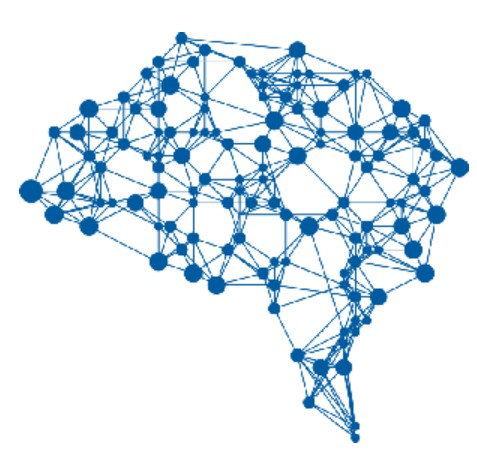
\includegraphics[scale=1]{0.DeepLearningLogo.jpg}
    \end{center}}



\begin{document}
\maketitle
\counterwithin{figure}{subsection}
\captionsetup[figure]{labelfont=bf}

\pagebreak

%% -- Sommario
\tableofcontents
\pagebreak


\section{Introduction to Artificial Neural Networks}

The lecture introduces the Multi-Layer Perceptron (MLP), covering its basic architecture,
the algebraic description of feed-forward networks, the Universal Approximation Theorems,
and the role of hidden layers in learning hierarchical representations.

\subsection{Recap: from Perceptrons to ANNs}

In previous lectures we saw that a single \textbf{perceptron} can implement simple logic gates.
However, using perceptrons directly for complex computations is inefficient: every new task requires
manual, ad-hoc tuning of the weights and biases.

The key insight is that we can build \textbf{learning algorithms}, i.e.\ Artificial Neural Networks (ANNs),
that automatically adjust the weights and biases of a network of artificial neurons.
This adjustment happens entirely in response to external data, with no direct human intervention at the
level of individual weights.

Three ingredients were necessary before real progress could be made:

\begin{enumerate}
    \item \textbf{Non-linearity.} For a network to \emph{learn}, a small change in a weight must produce a
          correspondingly small change in the output. Step functions (as used in the original perceptron)
          do not satisfy this requirement, because their output jumps abruptly. Smooth, differentiable
          activation functions (such as the sigmoid) solve this problem.
    \item \textbf{Backpropagation.} An efficient algorithm that computes the gradient of the loss function
          with respect to every weight in the network, enabling systematic weight updates.
    \item \textbf{Computational power.} Training large networks requires performing billions of
          floating-point operations, which only became feasible with modern hardware (GPUs, TPUs).
\end{enumerate}


\subsection{Multi-Layer Perceptron (MLP) Architecture}

\subsubsection{A Simple Layout}

\begin{defbox}{Feed-Forward Neural Network}
A \textbf{feed-forward neural network} (also called a Multi-Layer Perceptron, MLP) is a
network of artificial neurons organized in \textbf{layers}, where information flows in one
direction only: from the \textbf{input layer}, through one or more \textbf{hidden layers},
to the \textbf{output layer}. Neurons within the same layer are \emph{not} connected to each other;
each neuron connects only to neurons in the immediately subsequent layer.
\end{defbox}

     \begin{figure}[H] 
        \centering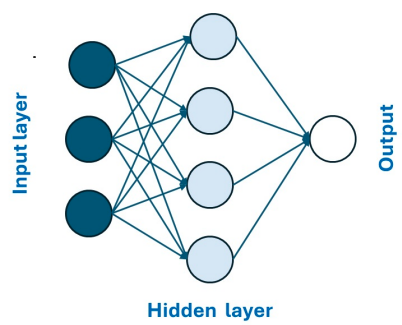
\includegraphics[scale=0.4]{6.Feed Forward Network.jpeg}
        \caption{Feed Forward Network}
    \captionsetup{font=footnotesize}
    \end{figure}

In a diagram each circle represents a neuron and each line represents a weighted connection.
The key properties of this layout are:

  

\begin{itemize}
    \item \textbf{Input layer:} receives the raw data (e.g.\ pixel values of an image). Each neuron
          holds one component of the input vector.
    \item \textbf{Hidden layer(s):} process the information coming from the previous layer.
          Each successive hidden layer builds higher-level, more abstract representations of the data.
    \item \textbf{Output layer:} produces the final prediction (e.g.\ a class label).
\end{itemize}

   


An important detail: the output of each neuron is \emph{unique}: that is, a neuron produces a
single scalar value, and that same value is sent to \emph{all} neurons in the next layer.


\subsubsection{The Mathematics of Data Flow (Forward Propagation)}
A fully connected neural network transforms input data layer by layer. Regardless of how deep the network is, every single hidden layer performs the exact same two-step mathematical operation.

Let $L^h$ be a hidden layer, $\mathbf{a}^{(h)}$ be its activation vector, $\mathbf{W}^{(h)}$ the weight matrix connecting it to the next layer, and $\mathbf{b}^{(h)}$ the bias vector.

\paragraph*{Step 1: Pre-Activation (Linear Transformation)}.
For the next layer $h+1$, we first compute the \textbf{pre-activation vector} ($\mathbf{z}$). This is simply the dot product of the weights and the previous layer's activations, plus the bias:
\begin{equation}
    \mathbf{z}^{(h+1)} = \mathbf{W}^{(h)} \mathbf{a}^{(h)} + \mathbf{b}^{(h)}
\end{equation}

\paragraph*{Step 2: Activation (Non-Linearity)}.
We then apply a differentiable, non-linear \textbf{activation function} ($\sigma$) element-wise to the pre-activation vector to get the final \textbf{activation vector} ($\mathbf{a}$):
\begin{equation}
    \mathbf{a}^{(h+1)} = \sigma\!\left(\mathbf{z}^{(h+1)}\right)
\end{equation}

\begin{figure}[H] 
    \centering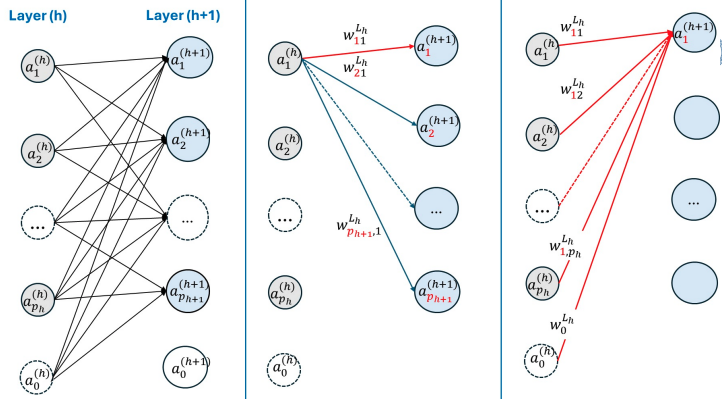
\includegraphics[scale=0.45]{7.neural network scheme.jpeg}
    \caption{Neural Network scheme}
\captionsetup{font=footnotesize}
\end{figure}

\subsubsection{The Network as a Function Composition}
Because every layer performs these same two steps, an entire deep neural network can be written as one massive nested mathematical function. If $\mathbf{x}$ is our input data, the final output $\mathbf{O}$ is:

\begin{equation}
    \mathbf{O} = \sigma_L\!\Bigl(\dots \sigma_2\!\bigl(\mathbf{W}^{(2)}\sigma_1\!\bigl(\mathbf{W}^{(1)}\mathbf{x} + \mathbf{b}^{(1)}\bigr) + \mathbf{b}^{(2)}\bigr)\dots\Bigr)
\end{equation}

\textbf{Why is the Activation Function ($\sigma$) strictly necessary?} \\
If we removed the non-linear $\sigma$, the network would just be a series of matrix multiplications: $\mathbf{W}^{(3)}(\mathbf{W}^{(2)}(\mathbf{W}^{(1)}\mathbf{x}))$. In linear algebra, multiplying multiple matrices just results in one single new matrix. Therefore, without non-linearity, a 100-layer deep neural network mathematically collapses into a basic linear regression model, entirely losing its ability to learn complex, curved boundaries.

\subsubsection{Network Design: Parameters vs. Hyperparameters}
When building these networks, a Data Scientist must clearly distinguish between what the machine learns and what the human decides:

\begin{itemize}
    \item \textbf{Parameters (Learned by the machine):} The actual numerical values inside the weight matrices ($\mathbf{W}$) and bias vectors ($\mathbf{b}$). These are automatically adjusted by the Backpropagation algorithm during training.
    \item \textbf{Hyperparameters (Set by the human):} The architectural design choices made \textit{before} training begins. This includes the number of hidden layers, the number of neurons in each layer, the learning rate, and the choice of activation functions (e.g., ReLU vs. Sigmoid).
\end{itemize}






%==========================================================
\subsubsection{Universal Approximation Theorems}
%==========================================================

These theorems provide a mathematical justification for using neural networks, assuring researchers that a sufficiently large or deep network can model the complex, non linear relationships often found in real-world data. 

\begin{defbox}{Universal Approximation Theorem (Hornik et al., 1988)}
A feed-forward neural network with a single hidden layer and a non-polynomial activation
function (e.g.\ sigmoid, ReLU) can approximate any continuous function on a compact
subset of $\mathbb{R}^n$ to any desired degree of accuracy, provided the hidden layer has
sufficiently many neurons.
\end{defbox}

There are two flavors of this result:

\begin{enumerate}
    \item \textbf{Width approach:} keep the network shallow (one hidden layer) but make it
          \emph{wider} by increasing the number of neurons in that layer.
    \item \textbf{Depth approach:} keep the width fixed but make the network \emph{deeper}
          by adding more hidden layers.
\end{enumerate}

Both strategies can achieve universal approximation in theory.

These are \textbf{existence theorems}. They guarantee that a network with the right
structure \emph{exists}, but they say nothing about:
\begin{itemize}
    \item how many neurons/layers are actually needed,
    \item how to find the correct values of the weights.
    \item whether gradient-based optimization will converge to the optimal solution.
\end{itemize}

In practice, finding good weights is the hard part and that is the job of training algorithms like backpropagation combined with gradient descent.

\subsubsection{The Power of Hidden Layers: Feature Hierarchies}

Why do we need hidden layers at all? The answer lies in the concept of \textbf{hierarchical
abstraction}.

\begin{defbox}{Hierarchical Feature Learning}
Hidden layers allow the network to learn a \textbf{hierarchy of representations} from the data.
Layers closer to the input learn simple, low-level features (e.g.\ edges, basic shapes),
while layers closer to the output learn complex, high-level features (e.g.\ object parts,
entire objects).
\end{defbox}

This principle applies across different data modalities:

\begin{itemize}
    \item \textbf{Images:} an image is composed of objects, which are composed of parts, which are
          composed of edges and textures. Early layers detect edges; middle layers detect shapes
          (e.g.\ loops, strokes); later layers detect complete objects (e.g.\ digits).
    \item \textbf{Text:} a sentence is composed of words, which are composed of syllables, which are
          composed of characters. Each level follows specific patterns that the network can learn.
    \item \textbf{Sound:} audio is composed of musical phrases, which are composed of notes organized
          at different levels.
\end{itemize}

\subsection{Analyzing a Simple MLP: The XOR Forward Pass}

\subsubsection{The XOR Problem Revisited}

The XOR function takes two binary inputs and returns:
\begin{itemize}
    \item \(1\) if the two inputs are different,
    \item \(0\) if the two inputs are equal.
\end{itemize}

Its truth table is:
\[
\begin{array}{c|c|c}
A & B & A \oplus B \\
\hline
0 & 0 & 0 \\
0 & 1 & 1 \\
1 & 0 & 1 \\
1 & 1 & 0
\end{array}
\]


As previously established, a single linear perceptron cannot solve the XOR logic gate because the data is not linearly separable. To solve it, we must build a \textbf{Multi-Layer Perceptron (MLP)} with at least one hidden layer. 



\subsubsection{Network Architecture \& Dimensionality}
Understanding matrix dimensions is the most critical skill for coding neural networks. Our XOR network is structured as follows:


\begin{figure}[H] 
    \centering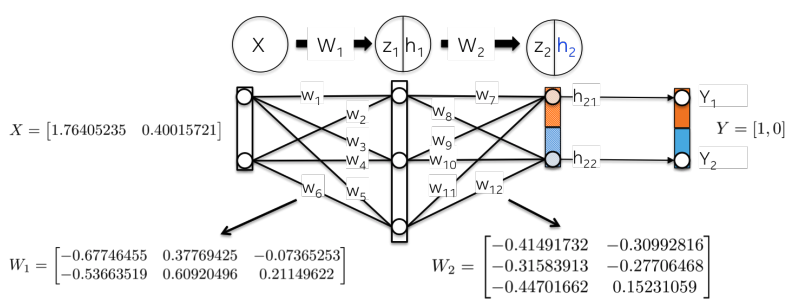
\includegraphics[scale=0.5]{8.Schematic layout of MLP.jpeg}
    \caption{Schematic layout of MLP}
\captionsetup{font=footnotesize}
\end{figure}

\begin{itemize}
    \item \textbf{Input ($X$):} 1 sample with 2 features. Dimension = $(1 \times 2)$.
    \item \textbf{Hidden Layer ($h_1$):} We choose 3 neurons. To get from 2 inputs to 3 neurons, our first weight matrix ($W_1$) must have the dimension $(2 \times 3)$.
    \item \textbf{Output Layer ($h_2$):} We need 2 outputs (for our one-hot classes). To get from 3 hidden neurons to 2 outputs, our second weight matrix ($W_2$) must be $(3 \times 2)$.
\end{itemize}




\subsubsection{The Forward Pass: Step-by-Step}
We will trace a single input vector $X = [1.76, 0.40]$ through the network to see how it transforms. (Note: Initial weights are chosen randomly).

\paragraph*{Step 1: Input to Hidden Layer (Linear)}.
We calculate the pre-activation $z_1$ by multiplying the input by the first weight matrix:
\[ z_1 = X \cdot W_1 \]
\[ (1 \times 2) \cdot (2 \times 3) \rightarrow \text{Resulting dimension is } (1 \times 3) \]
\textit{Data Science Takeaway:} The network has mathematically projected our 2D input into a new, 3-dimensional internal feature space.

\paragraph*{Step 2: Hidden Layer Activation (Non-Linear)}.
We apply the \textbf{Sigmoid Function} $\sigma(x) = \frac{1}{1+e^{-x}}$ element-wise to $z_1$. This squishes all three values into a range between 0 and 1, providing the crucial non-linearity. 
\[ h_1 = \sigma(z_1) = [0.19, \;\; 0.71, \;\; 0.48] \]

\paragraph*{Step 3: Hidden to Output Layer (Linear)}.
We take our new 3D feature vector ($h_1$) and multiply it by the second weight matrix to calculate the final pre-activation $z_2$:
\[ z_2 = h_1 \cdot W_2 \]
\[ (1 \times 3) \cdot (3 \times 2) \rightarrow \text{Resulting dimension is } (1 \times 2) \]
The result is $z_2 = [-0.52, \;\; -0.18]$. These are our raw output scores (logits).

\paragraph*{Step 4: Output Activation (Softmax)}.
We have two raw scores, but we want probabilities that sum to 100\% (1.0). We apply the \textbf{Softmax Function}:
\[ \text{Softmax}(z_i) = \frac{e^{z_i}}{\sum e^{z_j}} \]
\[ h_2 = \text{Softmax}([-0.52, -0.18]) = [0.37, \;\; 0.45] \text{ (Simplified for example)} \]


The network took the input $[1.76, 0.40]$ and predicted that it is roughly a 37\% match for Class 0, and a 45\% match for Class 1. 

Because the weights were initialized randomly, this prediction is essentially garbage. To make it accurate, the network would now calculate the Error (Loss) between this prediction and the true One-Hot target, and use \textbf{Backpropagation} to adjust $W_1$ and $W_2$.

\subsubsection{Why This Example Is Important}

This example is small, but it shows the essential logic of neural networks:
\begin{itemize}
    \item the input is multiplied by a weight matrix,
    \item the result is transformed through a non-linear activation function,
    \item the hidden representation is passed to another layer,
    \item the final output is converted into a probability-like vector.
\end{itemize}

Even though the network is simple, all larger MLPs work in the same general way.


\subsection{Backpropagation: The Backward Pass}

\subsubsection{The Goal of Backpropagation}
While the Forward Pass makes a prediction, the \textbf{Backward Pass} calculates exactly how wrong that prediction is and updates the network's weights to improve the next prediction. 

The algorithm that dictates this process is called \textbf{Backpropagation}. It computes the \textit{gradient} of the Loss function with respect to every single weight in the network, moving from the output layer backwards to the input layer.

\subsubsection{The Loss Function and Regularization}
Before we can backpropagate, we need to mathematically define our error using a \textbf{Loss Function} ($\mathcal{L}$). We can use as example Mean Squared Error (MSE) combined with Ridge ($\mathcal{L}^2$) Regularization:

\[
\mathcal{L} = \frac{1}{2N}\sum_{i=0}^{N}(y_i - h_{2i})^2 + \frac{\lambda}{2N}\sum_{j=0}^{M} W_j^2
\]

\begin{itemize}
    \item \textbf{Data Fitting Term (Left):} Measures the distance between the network's prediction ($h_2$) and the true label ($y$).
    \item \textbf{Regularization Term (Right):} Penalizes excessively large weights to prevent overfitting, controlled by the parameter $\lambda$.
\end{itemize}

\paragraph*{Step 1: Updating the Output Layer ($W_2$)}.
To update the weights connecting the hidden layer to the output layer ($W_2$), we must find the gradient $\frac{\partial \mathcal{L}}{\partial W_2}$. Because the network is a composite function ($h_1 \rightarrow z_2 \rightarrow h_2 \rightarrow \mathcal{L}$), we use the \textbf{Chain Rule}:

\[
\frac{\partial \mathcal{L}}{\partial W_2} = \frac{\partial \mathcal{L}}{\partial h_2} \cdot \frac{\partial h_2}{\partial z_2} \cdot \frac{\partial z_2}{\partial W_2}
\]

\begin{enumerate}
    \item \textbf{Loss Derivative} ($\frac{\partial \mathcal{L}}{\partial h_2}$): How the loss changes with respect to the final prediction.
    \item \textbf{Activation Derivative} ($\frac{\partial h_2}{\partial z_2}$): The slope of the Softmax/Sigmoid function.
    \item \textbf{Input Derivative} ($\frac{\partial z_2}{\partial W_2}$): The input to this layer, which is simply the activation of the previous hidden layer ($h_1$).
\end{enumerate}

Once we multiply these three terms together to get the gradient matrix, we apply \textbf{Gradient Descent} to update the weights, stepping in the opposite direction of the gradient by a factor of the learning rate ($\alpha$):

\[
W_2^{*} = W_2 - \alpha \frac{\partial \mathcal{L}}{\partial W_2}
\]

\paragraph*{Step 2: Updating the Hidden Layer ($W_1$)}.
Now we move backwards to the first weight matrix ($W_1$). The chain rule gets longer:


\begin{align*}
\frac{d\mathcal{L}}{dW_1}
&=
\frac{d\mathcal{L}}{dh_1}
\frac{dh_1}{dz_1}
\frac{dz_1}{dW_1}
\\[8pt]
\frac{d\mathcal{L}}{dh_1}
&=
\frac{d\mathcal{L}}{dz_2}
\frac{dz_2}{dh_1}
=
\frac{d\mathcal{L}}{dh_2}
\frac{dh_2}{dz_2}
\frac{dz_2}{dW_2}
\end{align*}


\[
\frac{\partial \mathcal{L}}{\partial W_1} = \left( \frac{\partial \mathcal{L}}{\partial h_2} \cdot \frac{\partial h_2}{\partial z_2} \cdot \frac{\partial z_2}{\partial h_1} \right) \cdot \frac{\partial h_1}{\partial z_1} \cdot \frac{\partial z_1}{\partial W_1}
\]

\vspace{0.25cm}
\textbf{Crucial Data Science Concept: Gradient Reuse}\\
Notice that the first two terms ($\frac{\partial \mathcal{L}}{\partial h_2} \cdot \frac{\partial h_2}{\partial z_2}$) are the exact same derivatives we calculated for $W_2$. The absolute genius of the Backpropagation algorithm is that \textbf{we do not recompute them}. We store the gradients from the later layers and reuse them for the earlier layers. This makes training deep networks computationally efficient.

Once the full gradient is calculated, we update the first matrix just like the second:
\[
W_1^{*} = W_1 - \alpha \frac{\partial \mathcal{L}}{\partial W_1}
\]

\paragraph*{Conclusion of the Training Step}.
By updating $W_2$ and then $W_1$, the network has completed one full learning cycle. The next time the identical input $X$ is passed forward, the new weights ($W_1^*$ and $W_2^*$) will produce an output that is slightly closer to the true target $Y$, resulting in a smaller Loss.

\subsection{The XOR Operator and General MLP Terminology}

\subsubsection{Why XOR Proves the Need for MLPs}
As demonstrated in the previous forward-pass example, the \textbf{XOR} (Exclusive OR) logical function cannot be solved by a single linear classifier because the classes are not linearly separable. 

This classical problem proved that artificial intelligence requires two things to solve complex real-world problems:
\begin{enumerate}
    \item \textbf{Hidden Layers:} To project the input data into a new, higher-dimensional space where the classes \textit{can} be separated.
    \item \textbf{Non-Linear Activation Functions:} To ensure that the multiple layers do not mathematically collapse back into a single linear equation.
\end{enumerate}

\subsubsection{The Multi-Layer Perceptron (MLP)}
An MLP is the simplest and most foundational type of Artificial Neural Network (ANN). It is a \textbf{Feed-Forward Network}, meaning data only moves in one direction (from left to right) without any loops or feedback cycles.

\vs
\textbf{Structural Terminology}
\begin{itemize}
    \item \textbf{Neuron (Node):} The basic computational unit. It takes inputs, multiplies them by weights, adds a bias, and passes the sum through an activation function to produce a single scalar output.
    \item \textbf{Layer:} A vertical column of neurons that operate in parallel. Neurons within the same layer do \textit{not} connect to each other.
    \item \textbf{Hidden Layer:} Any intermediate layer between the input and the output. It is "hidden" because the user never directly sees its values; it creates internal representations of the data.
    \item \textbf{Weights:} The numerical parameters connecting neurons across layers. \textit{These are the unknown variables that the network must learn.}
\end{itemize}

\begin{figure}[H] 
    \centering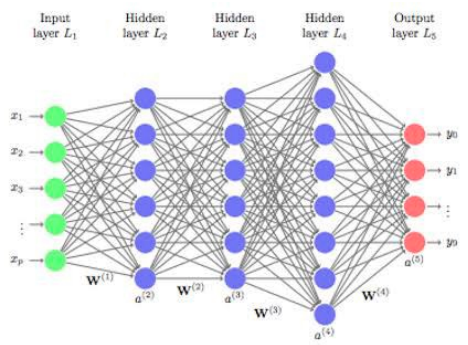
\includegraphics[scale=0.5]{9.Multi Layer Perceptron.jpeg}
    \caption{Multi Layer Perceptron}
\captionsetup{font=footnotesize}
\end{figure}

\subsubsection{The Knowledge Base: Managing Data in Machine Learning}
In Supervised Learning, the network learns from a \textbf{Knowledge Base}: a dataset containing input \textbf{Features} ($X$) paired with correct \textbf{Targets} ($Y$).

To properly train and evaluate a model without bias, a Data Scientist must split this knowledge base into three distinct subsets:

\begin{enumerate}
    \item \textbf{Training Set:} The data used to actually teach the model. The network makes predictions on this data, calculates the Cost (Loss) Function, and updates its weights via Backpropagation.
    \item \textbf{Validation Set:} A separate dataset used \textit{during} development. The model is evaluated on this set to help the data scientist tune \textbf{hyperparameters} (like learning rate or number of layers) and check for overfitting. The model does \textit{not} update its weights based on this data.
    \item \textbf{Test Set:} The final, untouched dataset. It is used only once at the very end of the project to evaluate how well the fully trained model \textbf{generalizes} to completely new, unseen data.
\end{enumerate}

\textbf{The Golden Rule of Data Science:} Never, under any circumstances, allow your model to train on or see the Test Set during the development phase.

\subsection{The Supervised Learning Workflow}

\subsubsection{The Machine Learning Pipeline}
Supervised learning is not just about the math of a neural network; it is a structured engineering pipeline. The workflow is divided into two distinct phases:

\pagebreak
\textbf{Phase 1: Training (Learning)}
\begin{enumerate}
    \item \textbf{Data Prep \& Split:} Collect a labeled \textit{Knowledge Base} and split it into a Training Set and a Test Set.
    \item \textbf{Normalization:} Rescale the input features (e.g., pixel values) to a standard range, usually between 0 and 1. This prevents large numbers from destabilizing the math.
    \item \textbf{Initialization:} Assign small, random starting values to all weights and biases. (If all weights started at 0, every neuron would learn the exact same thing).
    \item \textbf{Forward Pass:} Pass a batch of training data through the network to get a prediction.
    \item \textbf{Cost Calculation:} Use a Cost (Loss) Function to measure how wrong the prediction is compared to the true label.
    \item \textbf{Backpropagation \& Optimization:} Calculate the gradients and update the weights to reduce the error.
    \item \textbf{Iteration:} Repeat steps 4-6 thousands of times over the training set until a \textbf{Stopping Criterion} is met (e.g., the loss stops decreasing).
\end{enumerate}

\textbf{Phase 2: Inference (Production)}
Once the stopping criterion is met, training ends. The weights are locked in place, and the model is considered \textbf{frozen}. In the Inference phase, the frozen model is exposed to completely new, unseen data (the Test Set or real-world user data) to make final predictions.

\begin{figure}[H] 
    \centering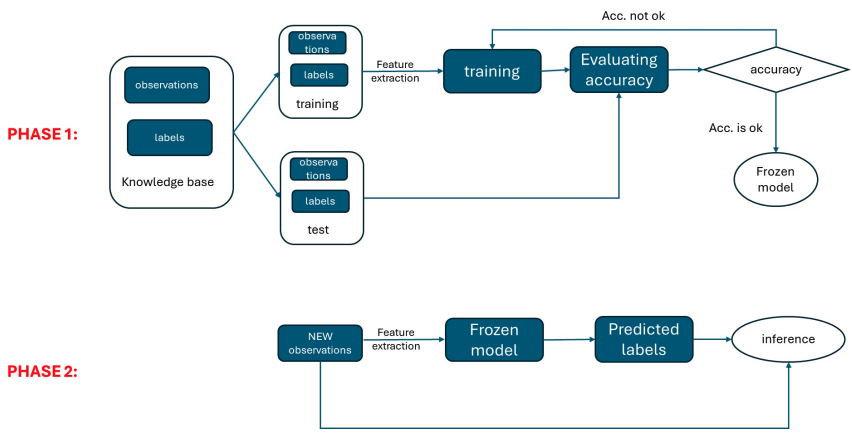
\includegraphics[scale=0.45]{10.Supervised Classification problem.jpeg}
    \caption{Supervised Classification problem}
\captionsetup{font=footnotesize}
\end{figure}

\subsubsection{Case Study: The MNIST Digit Classifier}
To make this abstract pipeline concrete, consider the classic "Hello World" of Deep Learning: classifying handwritten digits (0-9) from the MNIST dataset.

\paragraph*{Data Representation.}
Each MNIST image is a $28 \times 28$ pixel grayscale image. To feed this into a standard Feed-Forward network, the 2D image is \textit{flattened} into a single 1D vector of $784$ pixels.

\paragraph*{Network Architecture.}
The lecture proposes a specific architecture to solve this:
\[ 784 \text{ (Input)} \rightarrow 16 \text{ (Hidden)} \rightarrow 16 \text{ (Hidden)} \rightarrow 10 \text{ (Output)} \]
\begin{itemize}
    \item \textbf{Input Layer:} 784 neurons, one for each pixel.
    \item \textbf{Hidden Layers:} Two hidden layers with 16 neurons each to learn the shapes and curves of the numbers.
    \item \textbf{Output Layer:} 10 neurons, representing the probability of the image being the digit 0, 1, 2... up to 9. The neuron that "fires" the highest is the network's prediction.
\end{itemize}

\paragraph*{The Scale of Optimization.}
Even for this incredibly small, simple toy network, the math scales massively. 
\begin{itemize}
    \item Weights between Input and Hidden 1: $784 \times 16$
    \item Weights between Hidden 1 and Hidden 2: $16 \times 16$
    \item Weights between Hidden 2 and Output: $16 \times 10$
    \item Plus the biases for each layer ($16 + 16 + 10$)
\end{itemize}
Total Parameters to learn: \textbf{13,002}. 

\begin{figure}[H] 
    \centering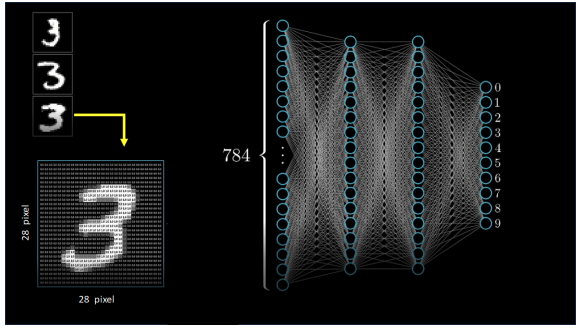
\includegraphics[scale=0.45]{11.The MNIST Digit Classifier.jpeg}
    \caption{The MNIST Digit Classifier}
\captionsetup{font=footnotesize}
\end{figure}

Training this network means finding the exact configuration of those 13,002 numbers that results in the lowest possible cost function. This is why automated algorithms like Backpropagation and powerful hardware like GPUs are absolutely mandatory for modern AI.



  \end{document}